% Drawing 67/05-5 -- folder 67, batch 05, archive page 97 (PDF page 98).
% Transcription: dans la marge gauche, à hauteur du cas hexagonal : un hexagone de sommets notés $v - u$, $v$, $u$, $u - v$, $-v$, $-u$, avec six flèches du centre vers les sommets, et au-dessus du côté du haut un triangle dont le sommet est noté $2v - u$.
% Kind: hexagon with named vertices, arrows from the centre, outer triangle with apex 2v-u. Method 2 (schematic redraw from the facsimile). Status: ok.
% Notes: As on the page: the six sides of the hexagon between the same six vertices, the six arrows from the centre to the vertices, the two sides of the outer triangle from the vertices v-u and v to the apex, and the seven labels where he wrote them (2v-u above the apex; v-u and v at the top; -u and u at the left and right; -v and u-v at the bottom). On the page the two sides of the outer triangle stop just short of the top side and of each other, and some sides are drawn in two strokes; the redraw joins them at the vertices. Redrawn 2026-11-12 (issue 128): to check again.
% Coordinates: 1 unit = 1 mm = 1/100 of the crop width (bbox in page fractions: [0.11, 0.4, 0.29, 0.54]).
% Redrawn by Claude (claude-fable-5-2), issue #128, 2026-11-12; not checked by a human; not compiled (no TeX in the session).
% Rights: reproduces part of the work -- behind RENDER_TRANSCRIPTS, never published by itself.
\documentclass[tikz,border=3pt]{standalone}
\usepackage{amsmath,amssymb}
\usetikzlibrary{patterns,arrows.meta}
\tikzset{pencil/.style={black!45}, struck/.style={black!35}, mpt/.style={circle,draw,inner sep=1.3pt}, pt/.style={circle,fill,inner sep=0.9pt}, opt/.style={circle,draw,fill=white,inner sep=1.1pt}}
\begin{document}
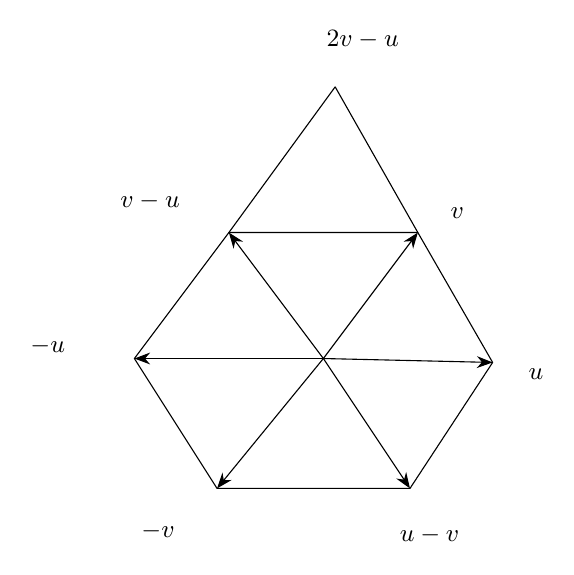
\begin{tikzpicture}[x=1mm,y=1mm,line cap=round,line join=round,font=\scriptsize]
\draw (47,-52.5) -- (71,-52.5) -- (80.5,-69) -- (70,-85) -- (45.5,-85) -- (35,-68.5) -- cycle;
\draw[-{Stealth[length=2mm]}] (59,-68.5) -- (47,-52.5);
\draw[-{Stealth[length=2mm]}] (59,-68.5) -- (71,-52.5);
\draw[-{Stealth[length=2mm]}] (59,-68.5) -- (80.5,-69);
\draw[-{Stealth[length=2mm]}] (59,-68.5) -- (70,-85);
\draw[-{Stealth[length=2mm]}] (59,-68.5) -- (45.5,-85);
\draw[-{Stealth[length=2mm]}] (59,-68.5) -- (35,-68.5);
\draw (47,-52.5) -- (60.5,-34) -- (71,-52.5);
\node[inner sep=1pt] at (64,-28) {\small $2v-u$};
\node[inner sep=1pt] at (37,-48.5) {\small $v-u$};
\node[inner sep=1pt] at (76,-50) {\small $v$};
\node[inner sep=1pt] at (24,-67) {\small $-u$};
\node[inner sep=1pt] at (86,-70.5) {\small $u$};
\node[inner sep=1pt] at (38,-90.5) {\small $-v$};
\node[inner sep=1pt] at (72.5,-91) {\small $u-v$};
\end{tikzpicture}
\end{document}
